\documentclass[report.tex]{subfiles}
\graphicspath{ \subfix{./images/} \subfix{./graphs/} }
\begin{document}
\section{Milestone 4: Handle data import/export}

\subsection{Implementation and testing}

I created a public static class in Algorithm Dynamics.Core project, so it is separated from the main UI logic and can be tested by the unit test framework. I set it as a static class since it is a collection of methods and no need of creating an instance.

I first created an ExportObject to wrap any data I am exporting, so the exported data can be validated before importing.

\begin{minted}{csharp}
/// <summary>
/// The base Object container that holds all the other data objects
/// It adds <see cref="FileType"/> and <see cref="DataType"/> info to the data.
/// </summary>
private class ExportObject
{
    public ExportObject(string dataType, object data)
    {
        DataType = dataType;
        Data = data;
    }

    public string FileType { get; set; } = "Algorithm Dynamics Exported Data";
    public string DataType { get; set; }
    public object Data { get; set; }
}
\end{minted}

The \code{ExportObject} adds \code{FileType} and \code{DataType} to the object, and store the actual instance in \code{Data}.

To export a problem, it is converted into an \code{ExportObject} and gets converted into a JSON string.

\begin{minted}{csharp}
/// <summary>
/// Convert a problem instance into a JSON string ready to be exported.
/// </summary>
/// <param name="problem"></param>
/// <returns></returns>
public static string SerializeProblem(Problem problem)
{
    return JsonSerializer.Serialize(new ExportObject("Problem", problem));
}
\end{minted}

Now I can add tests to Algorithm Dynamics.Test. The data serialization requires the database for the data model, so a new database is initialized for each test case at the beginning.

\begin{minted}{csharp}
using Algorithm_Dynamics.Core.Helpers;
using Algorithm_Dynamics.Core.Models;
using Microsoft.VisualStudio.TestTools.UnitTesting;
using System;
using System.IO;

namespace Algorithm_Dynamics.Test
{
    [TestClass]
    public class TestDataSerialization
    {
        [TestInitialize]
        public void InitDb()
        {
            string path = $"{Guid.NewGuid()}.db";
            File.Delete(path);
            DataAccess.InitializeDatabase(path);
        }

        [TestMethod]
        public void TestSerializeProblem()
        {
            Problem problem = DatabaseHelper.CreateFullProblem();
            
            // Serialize problem
            string str = DataSerialization.SerializeProblem(problem);

            Debug.WriteLine(str);
        }
    }
}
\end{minted}

When executing the test case, the following data is generated.

\begin{minted}{json}
{
    "FileType": "Algorithm Dynamics Exported Data",
    "DataType": "Problem",
    "Data": {
        "Id": 1,
        "Uid": "82a1ac35-f5bb-478f-8a36-50ffc03eab16",
        "Name": "Test Problem 1",
        "Description": "Description 1",
        "TimeLimit": 1000,
        "MemoryLimit": 16777216,
        "Status": 0,
        "StatusAsString": "Todo",
        "Difficulty": 0,
        "DifficultyAsString": "Easy",
        "TestCases": [
            {
                "Id": 1,
                "Input": "Input 3",
                "Output": "Output 3",
                "IsExample": true
            },
            {
                "Id": 2,
                "Input": "Input 5",
                "Output": "Output 5",
                "IsExample": true
            },
            {
                "Id": 3,
                "Input": "Input 7",
                "Output": "Output 7",
                "IsExample": true
            },
            {
                "Id": 4,
                "Input": "Input 9",
                "Output": "Output 9",
                "IsExample": true
            },
            {
                "Id": 5,
                "Input": "Input 11",
                "Output": "Output 11",
                "IsExample": true
            }
        ],
        "Tags": [
            {
                "Id": 1,
                "Name": "Tag 2"
            },
            {
                "Id": 2,
                "Name": "Tag 4"
            },
            {
                "Id": 3,
                "Name": "Tag 6"
            },
            {
                "Id": 4,
                "Name": "Tag 8"
            },
            {
                "Id": 5,
                "Name": "Tag 10"
            }
        ],
        "TagsAsString": "Tag 2, Tag 4, Tag 6, Tag 8, Tag 10",
        "TagAsString": "Tag 2"
    }
}
\end{minted}

The problem with all its metadata and all test cases and tags are exported correctly. However, some fields should not get exported. Such as \code{Id} and \code{Status}. Because when importing the data, all these fields will be regenerated any way, exporting them is just a waste of space.

I can add the \code{[JsonIgnore]} attribute to the fields that should not be exported.

Now when I test it again, only the necessary fields are exported.

\begin{minted}{json}
{
    "FileType": "Algorithm Dynamics Exported Data",
    "DataType": "Problem",
    "Data": {
        "Uid": "425f417f-0a9b-44e5-9e78-6c15d76ee4f2",
        "Name": "Test Problem 1",
        "Description": "Description 1",
        "TimeLimit": 1000,
        "MemoryLimit": 16777216,
        "Difficulty": 0,
        "TestCases": [
            {
                "Input": "Input 3",
                "Output": "Output 3",
                "IsExample": true
            },
            {
                "Input": "Input 5",
                "Output": "Output 5",
                "IsExample": true
            },
            {
                "Input": "Input 7",
                "Output": "Output 7",
                "IsExample": true
            },
            {
                "Input": "Input 9",
                "Output": "Output 9",
                "IsExample": true
            },
            {
                "Input": "Input 11",
                "Output": "Output 11",
                "IsExample": true
            }
        ],
        "Tags": [
            {
                "Name": "Tag 2"
            },
            {
                "Name": "Tag 4"
            },
            {
                "Name": "Tag 6"
            },
            {
                "Name": "Tag 8"
            },
            {
                "Name": "Tag 10"
            }
        ]
    }
}
\end{minted}

I implemented a similar export function for exporting a problem list.

\begin{minted}{csharp}
/// <summary>
/// Convert a problem list instance into a JSON string ready to be exported.
/// </summary>
/// <param name="problemList"></param>
/// <returns></returns>
public static string SerializeProblemList(ProblemList problemList)
{
    return JsonSerializer.Serialize(new ExportObject("ProblemList", problemList));
}
\end{minted}

And similarly, I add a test case for the problem list.

\begin{minted}{csharp}
[TestMethod]
public void TestSerializeProblemList()
{
    ProblemList problemList = DatabaseHelper.CreateFullProblemList();
    
    // Serialize problem list
    string str = DataSerialization.SerializeProblemList(problemList);

    Debug.WriteLine(str);
}
\end{minted}

When running the test, the problem list is exported correctly, with only necessary fields.

\begin{minted}{json}
{
    "FileType": "Algorithm Dynamics Exported Data",
    "DataType": "ProblemList",
    "Data": {
        "Name": "Problem List 1",
        "Description": "Description 1",
        "Problems": [
            {
                "Uid": "cd6edee3-479c-4833-b8b3-7aa955514cba",
                "Name": "Test Problem 2",
                "Description": "Description 2",
                "TimeLimit": 2000,
                "MemoryLimit": 33554432,
                "Difficulty": 0,
                "TestCases": [
                    {
                        "Input": "Input 4",
                        "Output": "Output 4",
                        "IsExample": true
                    },
                    {
                        "Input": "Input 6",
                        "Output": "Output 6",
                        "IsExample": true
                    }
                ],
                "Tags": [
                    {
                        "Name": "Tag 3"
                    },
                    {
                        "Name": "Tag 5"
                    }
                ]
            },
            {
                "Uid": "e207230d-a10d-4f76-bf5c-08273687dacc",
                "Name": "Test Problem 13",
                "Description": "Description 13",
                "TimeLimit": 13000,
                "MemoryLimit": 218103808,
                "Difficulty": 0,
                "TestCases": [
                    {
                        "Input": "Input 15",
                        "Output": "Output 15",
                        "IsExample": true
                    },
                    {
                        "Input": "Input 17",
                        "Output": "Output 17",
                        "IsExample": true
                    }
                ],
                "Tags": [
                    {
                        "Name": "Tag 14"
                    },
                    {
                        "Name": "Tag 16"
                    }
                ]
            }
        ]
    }
}
\end{minted}

Now, the export function is implemented and tested. To import the data, the data type is first checked and validated, then it is passed to the corresponding function to deserialize into an instance of the object.

I create a \code{GetDataType} function to retrieve the data type and validate the file format.

\begin{minted}{csharp}
/// <summary>
/// Get data type (problem/problem list) of an import data file.
/// </summary>
/// <param name="str"></param>
/// <returns></returns>
/// <exception cref="FormatException">The data format is invalid</exception>
public static string GetDataType(string str)
{
    var @base = JsonSerializer.Deserialize<ExportObject>(str);
    if (@base.FileType != "Algorithm Dynamics Exported Data")
        throw new FormatException($"The FileType {@base.FileType} is invalid.");

    if (@base.DataType != "Problem" && @base.DataType != "ProblemList")
        throw new FormatException($"The DataType {@base.DataType} is invalid.");
    return @base.DataType;
}
\end{minted}

\code{GetDataType} should throw \code{FormatException} whenever the file format is invalid. I added two tests to test the exceptions.

\begin{minted}{csharp}
[TestMethod, TestCategory("TestFormatException")]
[ExpectedException(typeof(FormatException))]
public void TestInvalidFileType()
{
    DataSerialization.GetDataType("{\"FileType\":\"Wrong Data\",\"DataType\":\"Problem\",\"Data\":{}}");
}

[TestMethod, TestCategory("TestFormatException")]
[ExpectedException(typeof(FormatException))]
public void TestInvalidDataType()
{
    DataSerialization.GetDataType("{\"FileType\":\"Algorithm Dynamics Exported Data\",\"DataType\":\"Wrong Data Type\",\"Data\":{}}");
}
\end{minted}

They each have an incorrect data type or file type, and a \code{FormatException} is thrown.

\begin{minted}{text}
> dotnet test --filter TestCategory=TestFormatException
  Determining projects to restore...
  All projects are up-to-date for restore.
  Algorithm Dynamics.Core -> C:\Algorithm-Dynamics\src\Algorithm Dynamics.Core\bin\Debug\net6.0\Algorithm Dynamics.Core.dll
  Algorithm Dynamics.Test -> C:\Algorithm-Dynamics\src\Algorithm Dynamics.Test\bin\Debug\net6.0\Algorithm Dynamics.Test.dll
Test run for C:\Algorithm-Dynamics\src\Algorithm Dynamics.Test\bin\Debug\net6.0\Algorithm Dynamics.Test.dll (.NETCoreApp,Version=v6.0)
Microsoft (R) Test Execution Command Line Tool Version 17.0.0
Copyright (c) Microsoft Corporation.  All rights reserved.

Starting test execution, please wait...
A total of 1 test files matched the specified pattern.

Passed!  - Failed:     0, Passed:     2, Skipped:     0, Total:     2, Duration: 204 ms - Algorithm Dynamics.Test.dll (net6.0)
\end{minted}

Both tests are passed successfully.

To deserialize the data, I need to first retrieve the data from the \code{ExportObject} instance and return it to the caller.

\begin{minted}{csharp}
/// <summary>
/// Convert a valid JSON string into a problem
/// </summary>
/// <param name="str"></param>
/// <returns></returns>
public static Problem DeserializeProblem(string str)
{
    // Convert the string into the base model
    var @base = JsonSerializer.Deserialize<ExportObject>(str);

    // Read the problem data from the base data
    var problem = JsonSerializer.Deserialize<Problem>(@base.Data.ToString());

    return problem;
}
\end{minted}

Next, I add a full test case for serializing and deserializing a problem.

\begin{minted}{csharp}
[TestMethod]
public void TestSerializeProblem()
{
    Problem problem = DatabaseHelper.CreateFullProblem();
    
    // Serialize problem
    string str = DataSerialization.SerializeProblem(problem);

    // Check data type
    Assert.AreEqual("Problem", DataSerialization.GetDataType(str));

    // Deserialize problem
    Problem result = DataSerialization.DeserializeProblem(str);
    
    // Check properties
    Assert.AreNotEqual(result.Id, problem.Id);
    Assert.AreEqual(result.Uid, problem.Uid);
    Assert.AreEqual(problem.Name, result.Name);
    Assert.AreEqual(problem.Description, result.Description);
    Assert.AreEqual(problem.TimeLimit, result.TimeLimit);
    Assert.AreEqual(problem.MemoryLimit, result.MemoryLimit);
    Assert.AreEqual(problem.Difficulty, result.Difficulty);
    
    // Check tags
    Assert.AreEqual(problem.Tags.Count, result.Tags.Count);
    for (int i = 0; i < problem.Tags.Count; i++)
    {
        Assert.AreEqual(problem.Tags[i].Name, result.Tags[i].Name);
    }
    
    // Check test cases
    Assert.AreEqual(problem.TestCases.Count, result.TestCases.Count);
    for (int i = 0; i < problem.TestCases.Count; i++)
    {
        Assert.AreEqual(problem.TestCases[i].Input, result.TestCases[i].Input);
        Assert.AreEqual(problem.TestCases[i].Output, result.TestCases[i].Output);
    }
}
\end{minted}

It generates a new problem, serializes it into a JSON string, deserializes from the JSON string into an instance, and compare the new instance and the original instance. The test passes when they are the same.

However, when I run the test, it fails with the following error.

\begin{minted}{text}
Message: 
Test method Algorithm_Dynamics.Test.TestDataSerialization.TestSerializeProblem threw exception: 
System.NotSupportedException: Deserialization of types without a parameterless constructor, a singular parameterized constructor, or a parameterized constructor annotated with 'JsonConstructorAttribute' is not supported. Type 'Algorithm_Dynamics.Core.Models.Problem'. Path: $ | LineNumber: 0 | BytePositionInLine: 1. ---> System.NotSupportedException: Deserialization of types without a parameterless constructor, a singular parameterized constructor, or a parameterized constructor annotated with 'JsonConstructorAttribute' is not supported. Type 'Algorithm_Dynamics.Core.Models.Problem'.

Stack Trace: 
ThrowHelper.ThrowNotSupportedException(ReadStack& state, Utf8JsonReader& reader, NotSupportedException ex)
ThrowHelper.ThrowNotSupportedException_DeserializeNoConstructor(Type type, Utf8JsonReader& reader, ReadStack& state)
ObjectDefaultConverter`1.OnTryRead(Utf8JsonReader& reader, Type typeToConvert, JsonSerializerOptions options, ReadStack& state, T& value)
JsonConverter`1.TryRead(Utf8JsonReader& reader, Type typeToConvert, JsonSerializerOptions options, ReadStack& state, T& value)
JsonConverter`1.ReadCore(Utf8JsonReader& reader, JsonSerializerOptions options, ReadStack& state)
JsonSerializer.ReadFromSpan[TValue](ReadOnlySpan`1 utf8Json, JsonTypeInfo jsonTypeInfo, Nullable`1 actualByteCount)
JsonSerializer.ReadFromSpan[TValue](ReadOnlySpan`1 json, JsonTypeInfo jsonTypeInfo)
JsonSerializer.Deserialize[TValue](String json, JsonSerializerOptions options)
DataSerialization.DeserializeProblem(String str) line 117
TestDataSerialization.TestSerializeProblem() line 32
\end{minted}

The deserializer requires a custom constructor to create an object. Instead of changing the existing design of the Problem model. I decided to create a base problem model to retrieve the data, and then convert the base mode into a full problem model.

\begin{minted}{csharp}
/// <summary>
/// The base test case model to hold the import data.
/// </summary>
private class BaseTestCase
{
    public string Input { get; set; }
    public string Output { get; set; }
    public bool IsExample { get; set; }
}

/// <summary>
/// The base tag model to hold the import data.
/// </summary>
private class BaseTag
{
    public string Name { get; set; }
}

/// <summary>
/// The base problem model to hold the import data
/// </summary>
private class BaseProblem
{
    public string Uid { get; set; }
    public string Name { get; set; }
    public string Description { get; set; }
    public int TimeLimit { get; set; }
    public int MemoryLimit { get; set; }
    public int Difficulty { get; set; }
    public List<BaseTestCase> TestCases { get; set; }
    public List<BaseTag> Tags { get; set; }
}
\end{minted}

These base models only have the fields that get exported. I decide to set them as private classes since it is only used for the deserializer internally, other classes do not need to access it. The deserializer first saves the data into the base problem model.

\begin{minted}{csharp}
public static Problem DeserializeProblem(string str)
{
    // Convert the string into the base model
    var @base = JsonSerializer.Deserialize<ExportObject>(str);

    // Read the problem data from the base data
    var baseProblem = JsonSerializer.Deserialize<BaseProblem>(@base.Data.ToString());
}
\end{minted}

Next, the data in the base model is used to create the actual problem model.

\begin{minted}{csharp}
// Create test cases and tags first
List<TestCase> testCases = new();
List<Tag> tags = new();
foreach (BaseTestCase t in baseProblem.TestCases)
{
    testCases.Add(TestCase.Create(t.Input, t.Output, t.IsExample));
}
foreach (BaseTag t in baseProblem.Tags)
{
    tags.Add(Tag.Create(t.Name));
}

// Create the problem next and return it
return Problem.Create(
    Guid.Parse(baseProblem.Uid),
    baseProblem.Name,
    baseProblem.Description,
    baseProblem.TimeLimit,
    baseProblem.MemoryLimit,
    (Difficulty)baseProblem.Difficulty,
    testCases,
    tags);
\end{minted}

Now I run the tests again, the test passed successfully.

\begin{minted}{text}
> dotnet test --filter TestCategory=TestSerialize
  Determining projects to restore...
  All projects are up-to-date for restore.
  Algorithm Dynamics.Core -> C:\Algorithm-Dynamics\src\Algorithm Dynamics.Core\bin\Debug\net6.0\Algorithm Dynamics.Core.dll
  Algorithm Dynamics.Test -> C:\Algorithm-Dynamics\src\Algorithm Dynamics.Test\bin\Debug\net6.0\Algorithm Dynamics.Test.dll
Test run for C:\Algorithm-Dynamics\src\Algorithm Dynamics.Test\bin\Debug\net6.0\Algorithm Dynamics.Test.dll (.NETCoreApp,Version=v6.0)
Microsoft (R) Test Execution Command Line Tool Version 17.0.0
Copyright (c) Microsoft Corporation.  All rights reserved.

Starting test execution, please wait...
A total of 1 test files matched the specified pattern.

Passed!  - Failed:     0, Passed:     1, Skipped:     0, Total:     1, Duration: 569 ms - Algorithm Dynamics.Test.dll (net6.0)
\end{minted}

I used a similar approach to handle the problem list. First, create the base problem list model.

\begin{minted}{csharp}
/// <summary>
/// The base problem list 
/// </summary>
private class BaseProblemList
{
    public string Name { get; set; }
    public string Description { get; set; }
    public List<BaseProblem> Problems { get; set; }
}
\end{minted}

Next, deserialize the base model and then create the actual model from the base model.

\begin{minted}{csharp}
/// <summary>
/// Convert a valid JSON string into a problem list
/// </summary>
/// <param name="str"></param>
/// <returns></returns>
public static ProblemList DeserializeProblemList(string str)
{
    // Convert the string into the base model
    var @base = JsonSerializer.Deserialize<ExportObject>(str);

    // Read the problem list data from the base data
    var baseProblemList = JsonSerializer.Deserialize<BaseProblemList>(@base.Data.ToString());
    List<Problem> problems = new();
    foreach (BaseProblem p in baseProblemList.Problems)
    {
        // Create problem from the problem list data
        List<TestCase> testCases = new();
        List<Tag> tags = new();
        foreach (BaseTestCase t in p.TestCases)
        {
            testCases.Add(TestCase.Create(t.Input, t.Output, t.IsExample));
        }
        foreach (BaseTag t in p.Tags)
        {
            tags.Add(Tag.Create(t.Name));
        }

        // Add to the problem list
        problems.Add(
            Problem.Create(
                Guid.Parse(p.Uid),
                p.Name,
                p.Description,
                p.TimeLimit,
                p.MemoryLimit,
                (Difficulty)p.Difficulty,
                testCases,
                tags
            )
        );
    }
    return ProblemList.Create(baseProblemList.Name, baseProblemList.Description, problems);
}
\end{minted}

Finally, add tests for the problem list.

\begin{minted}{csharp}
[TestMethod, TestCategory("TestSerialize")]
public void TestSerializeProblemList()
{
    ProblemList problemList = DatabaseHelper.CreateFullProblemList();
    
    // Serialize problem list
    string str = DataSerialization.SerializeProblemList(problemList);
    
    // Check data type
    Assert.AreEqual("ProblemList", DataSerialization.GetDataType(str));

    // Deserialize problem list
    ProblemList result = DataSerialization.DeserializeProblemList(str);
    
    // Check problem list metadata
    Assert.AreNotEqual(result.Id, problemList.Id);
    Assert.AreEqual(problemList.Name, result.Name);
    Assert.AreEqual(problemList.Description, result.Description);
    Assert.AreEqual(problemList.Problems.Count, result.Problems.Count);
    
    // Check problem data
    for (int i = 0; i < problemList.Problems.Count; i++)
    {
        var expected = problemList.Problems[i];
        var actual = result.Problems[i];
        Assert.AreNotEqual(expected.Id, actual.Id);
        Assert.AreEqual(expected.Uid, actual.Uid);
        Assert.AreEqual(expected.Name, actual.Name);
        Assert.AreEqual(expected.Description, actual.Description);
        Assert.AreEqual(expected.TimeLimit, actual.TimeLimit);
        Assert.AreEqual(expected.MemoryLimit, actual.MemoryLimit);
        Assert.AreEqual(expected.Difficulty, actual.Difficulty);
        
        // Check tag data
        Assert.AreEqual(expected.Tags.Count, actual.Tags.Count);
        for (int j = 0; j < expected.Tags.Count; j++)
        {
            Assert.AreEqual(expected.Tags[j].Name, actual.Tags[j].Name);
        }

        // Check test case data
        Assert.AreEqual(expected.TestCases.Count, actual.TestCases.Count);
        for (int j = 0; j < expected.TestCases.Count; j++)
        {
            Assert.AreEqual(expected.TestCases[j].Input, actual.TestCases[j].Input);
            Assert.AreEqual(expected.TestCases[j].Output, actual.TestCases[j].Output);
        }
    }
}
\end{minted}

Now when I run the tests, both of them passed successfully.

\begin{minted}{text}
> dotnet test --filter TestCategory=TestSerialize
  Determining projects to restore...
  All projects are up-to-date for restore.
  Algorithm Dynamics.Core -> C:\Algorithm-Dynamics\src\Algorithm Dynamics.Core\bin\Debug\net6.0\Algorithm Dynamics.Core.dll
  Algorithm Dynamics.Test -> C:\Algorithm-Dynamics\src\Algorithm Dynamics.Test\bin\Debug\net6.0\Algorithm Dynamics.Test.dll
Test run for C:\Algorithm-Dynamics\src\Algorithm Dynamics.Test\bin\Debug\net6.0\Algorithm Dynamics.Test.dll (.NETCoreApp,Version=v6.0)
Microsoft (R) Test Execution Command Line Tool Version 17.0.0
Copyright (c) Microsoft Corporation.  All rights reserved.

Starting test execution, please wait...
A total of 1 test files matched the specified pattern.

Passed!  - Failed:     0, Passed:     2, Skipped:     0, Total:     2, Duration: 1 s - Algorithm Dynamics.Test.dll (net6.0)
\end{minted}

\subsection{Integration}

Since the data serialization helper passes all the unit tests successfully, I am confident that it contains no issues and I can integrate them directly into the main project.

The user can import data from either the homepage or the problems page.

On the homepage, I add an action for the quick access item, which will be invoked when the user clicks the grid item.

\begin{minted}{csharp}
QAItems.Add(new QuickAccessItem("Import", Symbol.Import, async () =>
{
    IReadOnlyList<StorageFile> files = await FileHelper.FileOpenPicker(".json");
    if (files.Count > 0)
    {
        foreach (StorageFile file in files)
        {
            // Read data
            string data = await FileIO.ReadTextAsync(file);

            // Get data type
            string dataType = DataSerialization.GetDataType(data);

            // Deserialize the data and save to the database
            if (dataType == "Problem")
            {
                DataSerialization.DeserializeProblem(data);
            }
            else if (dataType == "ProblemList")
            {
                DataSerialization.DeserializeProblemList(data);
            }
        }
    }
\end{minted}

The \code{FileOpenPicker} is a helper function to open a Windows dialogue allowing the user to pick multiple JSON files.

\begin{minted}{csharp}
internal async static Task<IReadOnlyList<StorageFile>> FileOpenPicker(string fileTypeFilter = "*")
{
    // https://github.com/microsoft/WindowsAppSDK/issues/1188
    // https://docs.microsoft.com/en-us/windows/uwp/files/quickstart-using-file-and-folder-pickers
    var filePicker = new FileOpenPicker();

    // Get the current window's HWND by passing in the Window object
    var hwnd = WindowNative.GetWindowHandle(App.m_window);

    // Associate the HWND with the file picker
    InitializeWithWindow.Initialize(filePicker, hwnd);

    // Use file picker like normal!
    filePicker.FileTypeFilter.Add(fileTypeFilter);
    IReadOnlyList<StorageFile> files = await filePicker.PickMultipleFilesAsync();
    return files;
}
\end{minted}

Now when I click the import button on the HomePage, a dialogue shows up correctly.

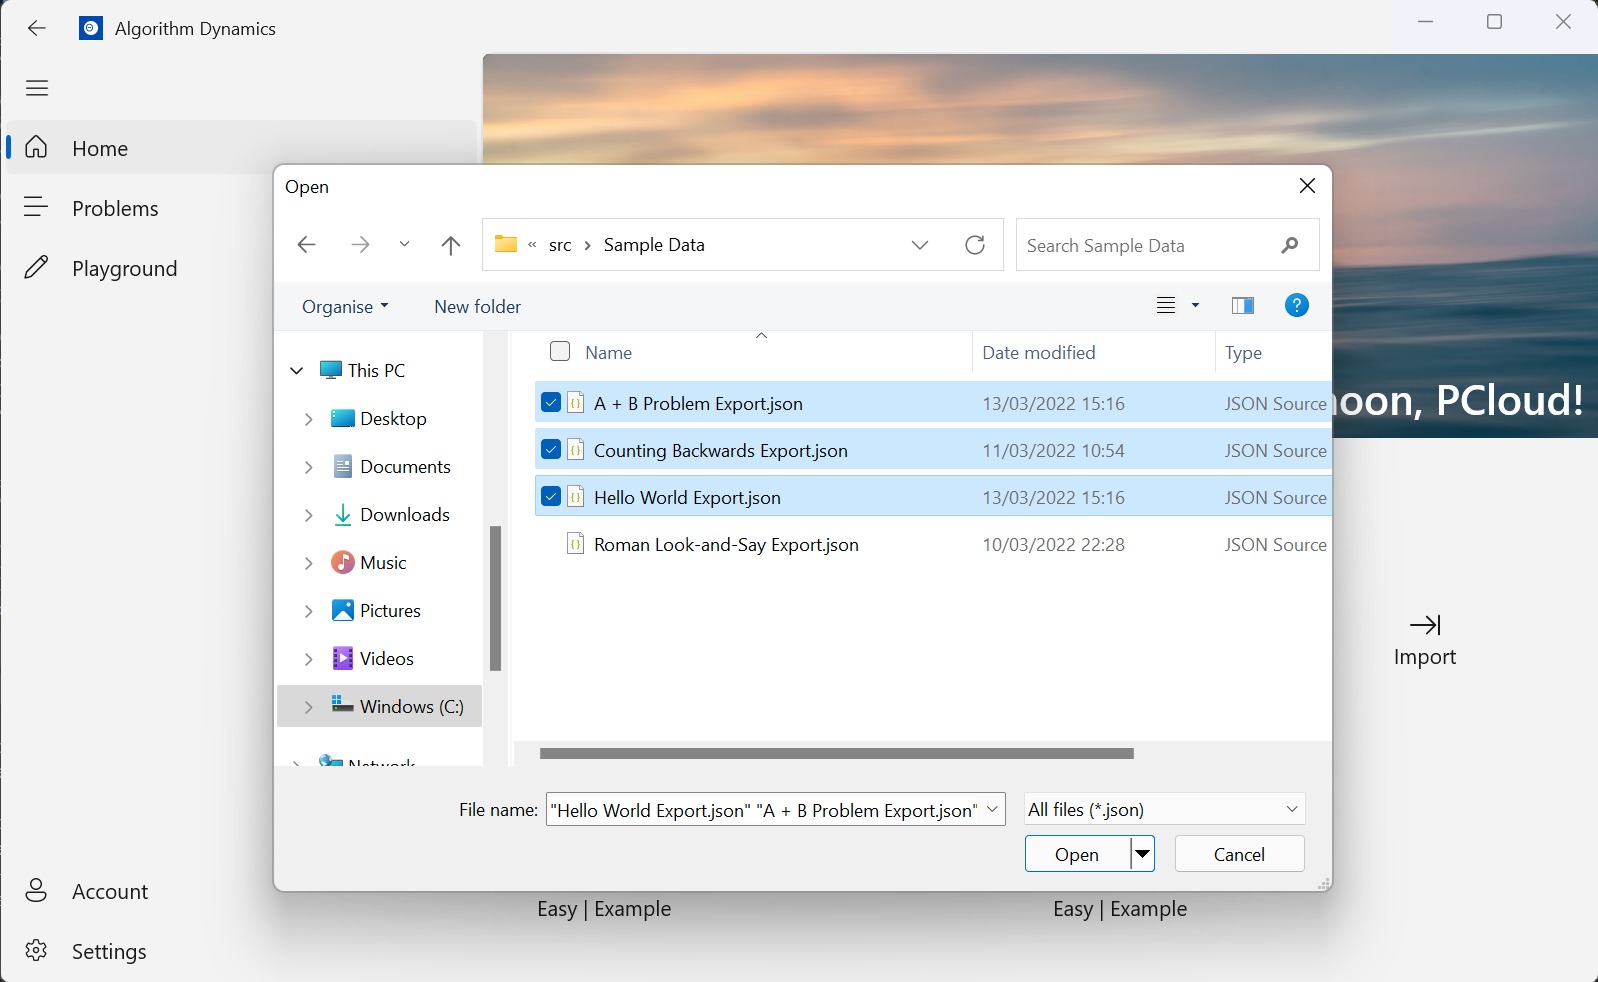
\includegraphics[width=\textwidth, height=\textheight, keepaspectratio]{HomePage-Import}

When I click open, the three problems are imported correctly.

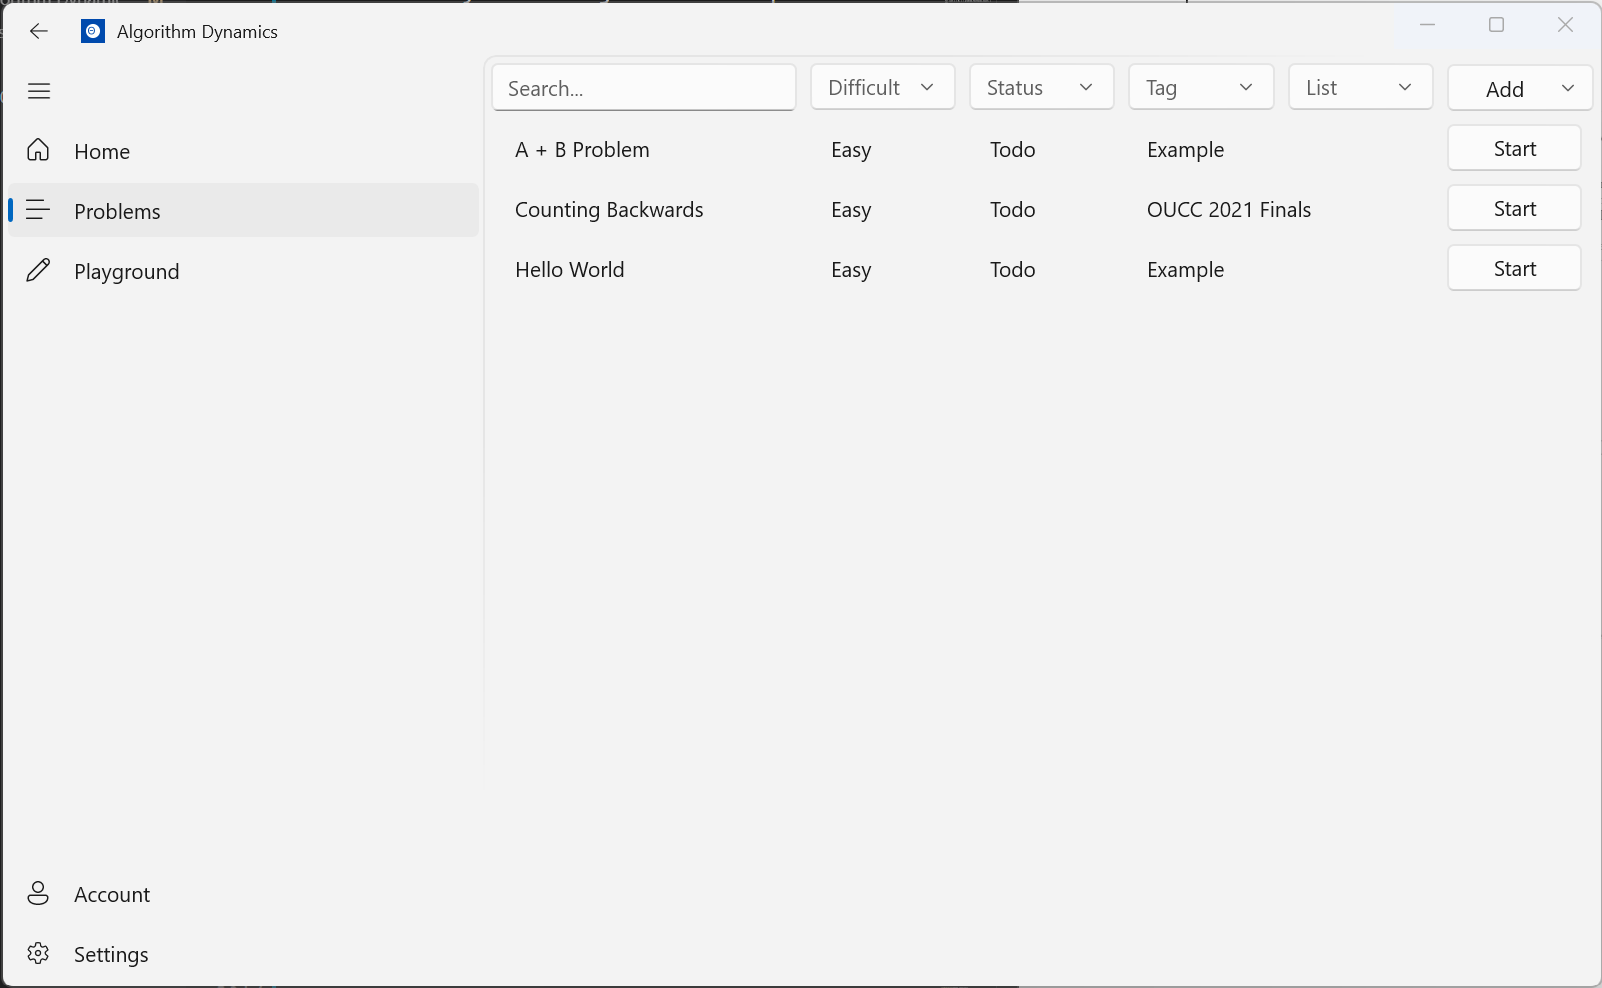
\includegraphics[width=\textwidth, height=\textheight, keepaspectratio]{ProblemsPage-Import}

However, when I try to import an invalid problem, the app crashes. This is expected behaviour since I have not handled the exception properly yet. I use a try-catch block to handle the exception. If any exception happens, a dialogue will show up and display the reason why the import is unsuccessful.

\begin{minted}{csharp}
try
{
    // Read data
    string data = await FileIO.ReadTextAsync(file);
    
    // Get data type
    string dataType = DataSerialization.GetDataType(data);

    // Deserialize the data and save to the database
    if (dataType == "Problem")
    {
        DataSerialization.DeserializeProblem(data);
    }
    else if (dataType == "ProblemList")
    {
        DataSerialization.DeserializeProblemList(data);
    }
}
catch (Exception e)
{
    // Show an dialog with the error message
    ContentDialog dialog = new()
    {
        Title = $"An error was encountered while importing {file.DisplayName}",
        PrimaryButtonText = "Ok",
        Content = $"The following error is encountered:\n\n{e.Message}",
        DefaultButton = ContentDialogButton.Primary,
        XamlRoot = Content.XamlRoot
    };
    await dialog.ShowAsync();
}
\end{minted}

Now, if I attempted to import something invalid, this dialogue will show up and abort the import.

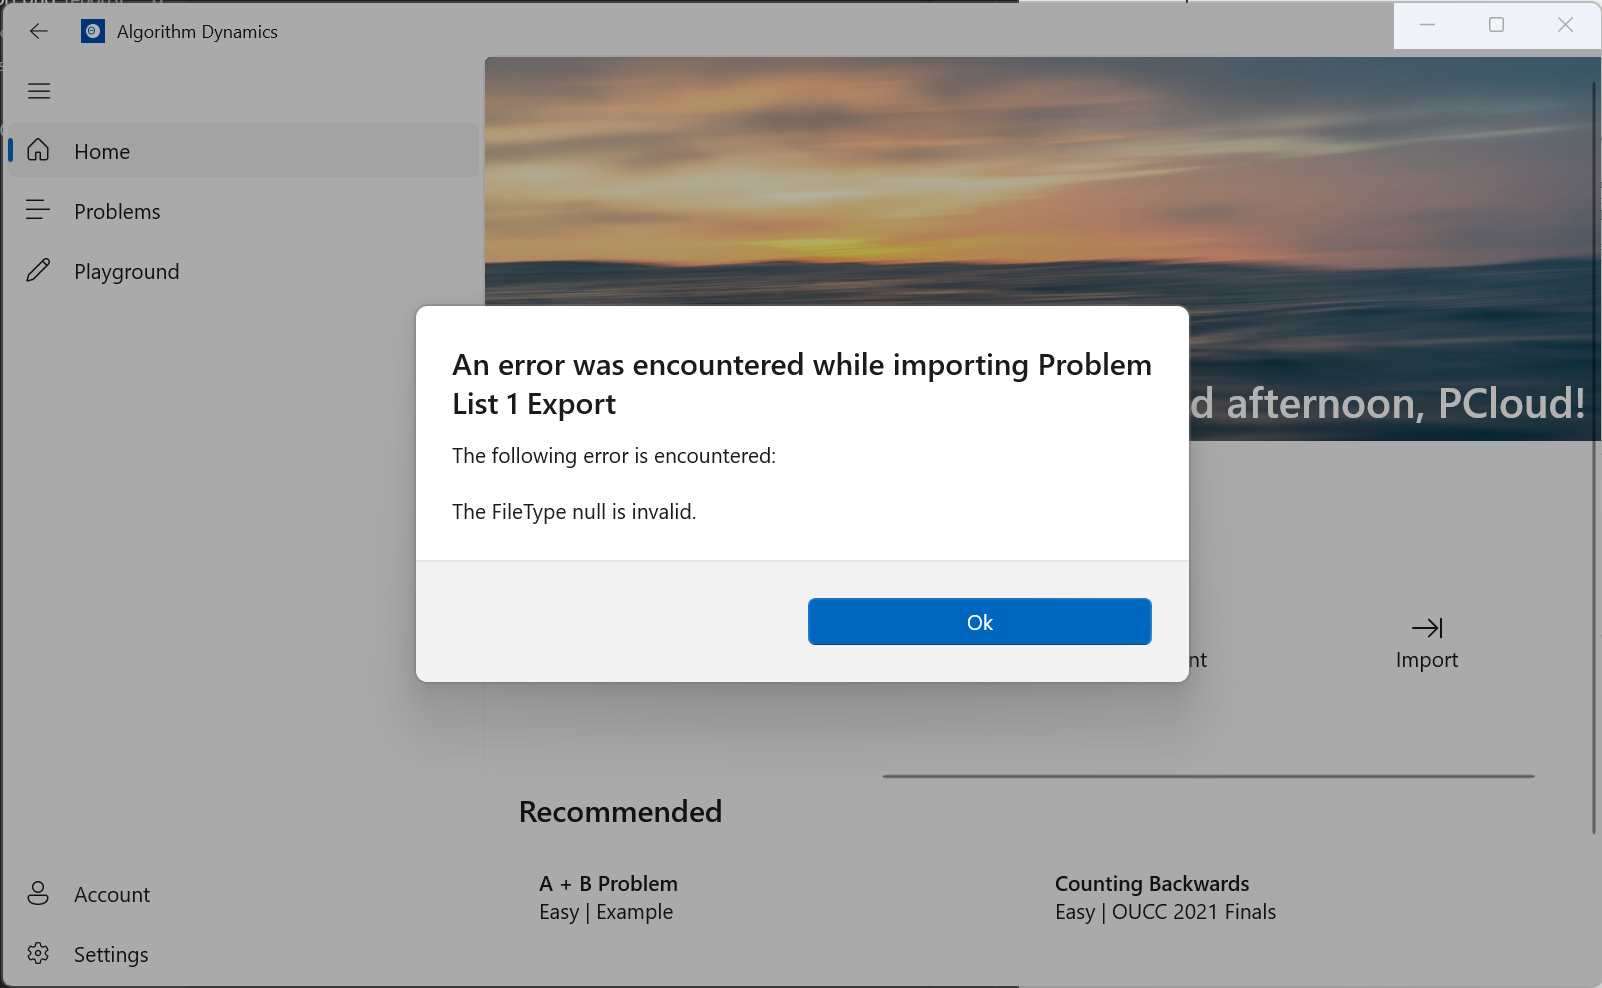
\includegraphics[width=\textwidth, height=\textheight, keepaspectratio]{HomePage-Import-Error}

I connect the same function to the import button on the ProblemsPage. The actual code is very similar so check out the \hyperref[subsubsec:problemspage]{source code} for details.

The user can export a problem or a problem list from the ProblemsPage.

\begin{minted}{csharp}
/// <summary>
/// Export problem to a JSON file
/// </summary>
/// <param name="sender"></param>
/// <param name="e"></param>
private async void ExportProblem(object sender, RoutedEventArgs e)
{
    // Get selected problem
    Problem problem = ProblemsListView.SelectedItem as Problem;
    
    // Set file name
    string fileName = $"{problem.Name} Export";
    
    // Serialize problem
    string serializedProblem = DataSerialization.SerializeProblem(problem);
    
    // Save problem
    await FileHelper.FileSavePicker("Algorithm Dynamics Export File", new() { ".json" }, fileName, serializedProblem);
}

/// <summary>
/// Export problem list to a JSON file
/// </summary>
/// <param name="sender"></param>
/// <param name="e"></param>
private async void ExportProblemList(object sender, RoutedEventArgs e)
{
    // Get selected problem list
    ProblemList problemList = ListComboBox.SelectedItem as ProblemList;
    
    // Set file name
    string fileName = $"{problemList.Name} Export";
    
    // Serialize problem
    string serializedProblem = DataSerialization.SerializeProblemList(problemList);
    
    // Save problem list
    await FileHelper.FileSavePicker("Algorithm Dynamics Export File", new() { ".json" }, fileName, serializedProblem);
}
\end{minted}

It is very easy to serialize the data since the data serialization helper I wrote before has done most of the work. I only need to read the selected problem, serialize it and save it to the disk.

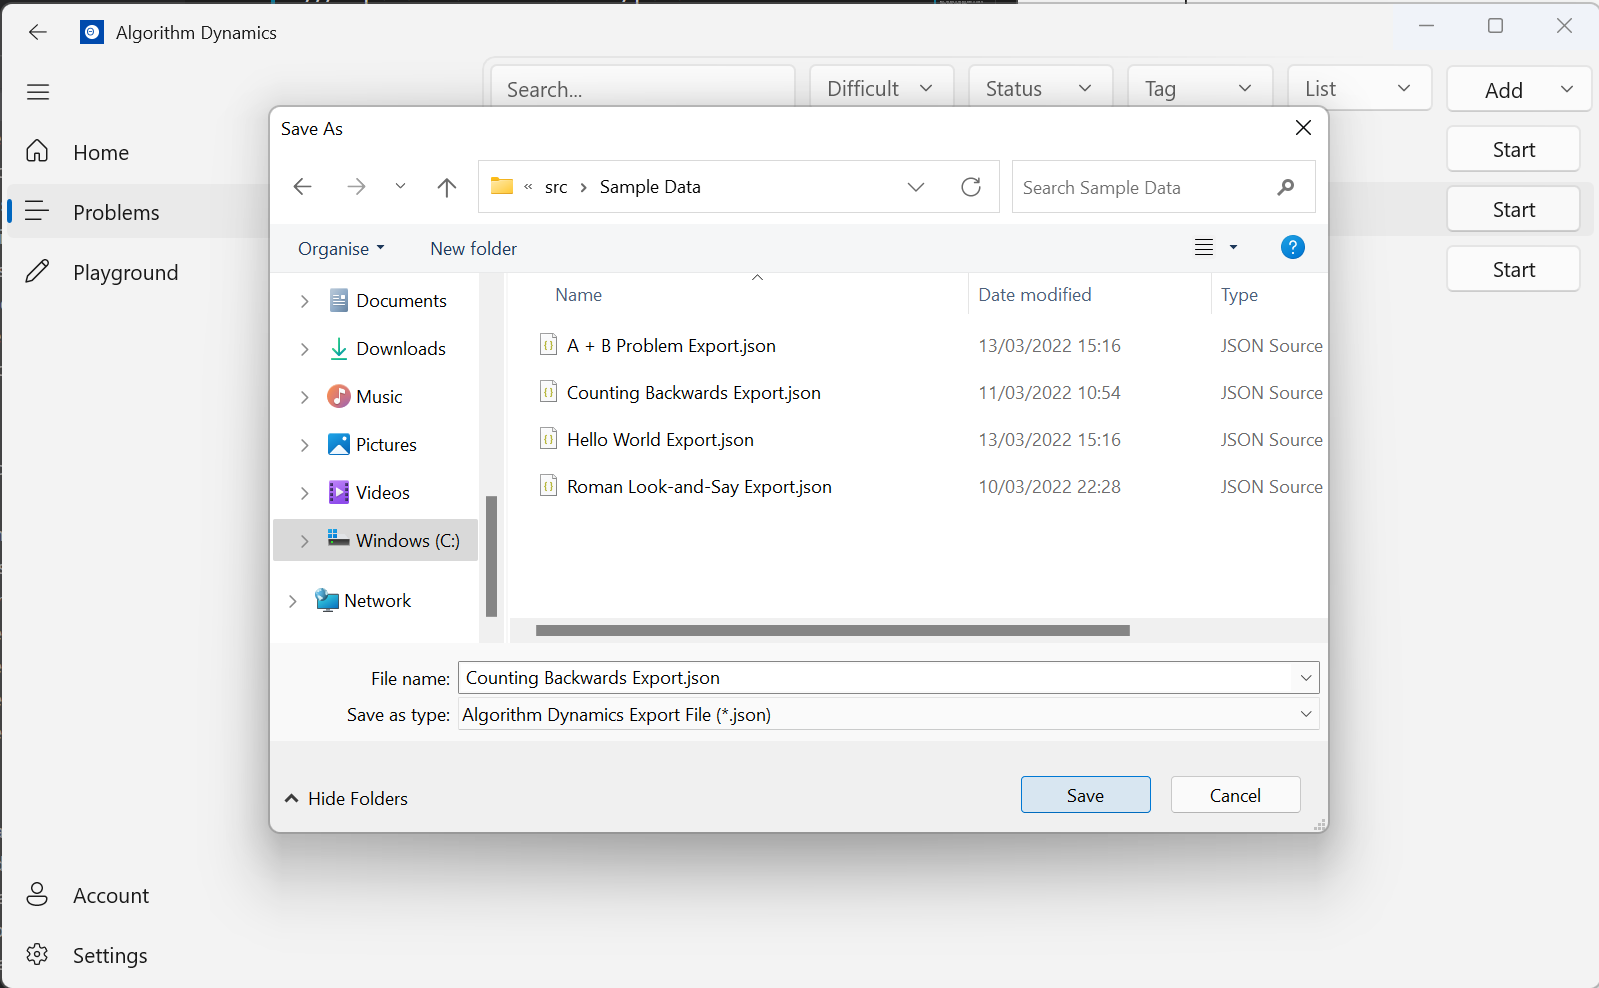
\includegraphics[width=\textwidth, height=\textheight, keepaspectratio]{ProblemsPage-Export}

The data is saved to the disk correctly after I click the save button.

The user can export the problem list directly from the CreateNewProblemListPage as well. The implementation is very similar, check out the source code for details.

\subsection{Stakeholder feedback}

I asked my stakeholders to test the data import/export function. They are pretty happy about its implementation. PCloud says that he is particularly satisfied because the speed of the import/export is very fast. He can import a large amount of data instantly. Timofei says he is happy about how the import is aborted and a useful error message is displayed when the data is invalid. Mr Grimwood suggests that the app should navigate to the ProblemsPage once the import on the homepage is completed, so he can check out the data he imports right away. I think this is a very sensible feature, and it is easy to implement.

\begin{minted}{csharp}
// Deserialize the data and save to the database
if (dataType == "Problem")
{
    DataSerialization.DeserializeProblem(data);
}
else if (dataType == "ProblemList")
{
    DataSerialization.DeserializeProblemList(data);
}

// Navigate to ProblemsPage on success
App.NavigateTo(typeof(ProblemsPage));
\end{minted}

Now the app will navigate the problem page when the import is completed. Mr Grimwood is satisfied with this feature.

\end{document}